\newpage
\section{ĐƯỜNG THẲNG TRONG MẶT PHẲNG TỌA ĐỘ}
\subsection{LÝ THUYẾT CẦN NHỚ}
\subsubsection{Vectơ chỉ phương và vectơ pháp tuyến của đường thẳng}
\begin{itemize}[\iconMT]
	\item Vectơ chỉ phương
	\immini{
		Vectơ $\overrightarrow{u} \ne \overrightarrow{0}$ được gọi là vectơ chỉ phương (VTCP) của đường thẳng $\Delta$ nếu giá của nó song song hoặc trùng với $\Delta$. Kí hiệu VTCP $\overrightarrow{u}_{\Delta}$.}
	{
		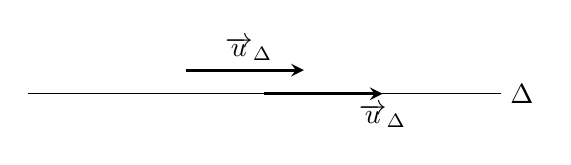
\begin{tikzpicture}[scale=1, >= stealth]
			\draw (0,0)--(6,0) node[right] {$\Delta$} ;
			\draw[->,line width =1pt] (3,0)--(4.5,0)  node[below] {$\overrightarrow{u}_{\Delta}$} ;
			\draw[->,line width =1pt] (2,0.3)--(3.5,0.3) ; 
			\draw (2.8,0.3)node[above] {$\overrightarrow{u}_{\Delta}$} ;
		\end{tikzpicture}
	}
	\item Vectơ pháp tuyến
	\immini{
		Vectơ $\overrightarrow{n} \ne \overrightarrow{0}$ được gọi là vectơ pháp tuyến  (VTPT) của đường thẳng $\Delta$ nếu giá của nó vuông góc với $\Delta$. Kí hiệu VTPT $\overrightarrow{n}_{\Delta}$.}
	{
		\begin{tikzpicture}[scale=1, >= stealth]
			\draw (0,0)--(6,0) node[right] {$\Delta$} ;
			\draw[->,line width =1pt] (4,0)--(4,1)  node[above] {$\overrightarrow{n}_{\Delta}$} ;
			\draw (3.8,0)|- (4,.2);
		\end{tikzpicture}
	}
\end{itemize}
\begin{luuy}
	\begin{itemize}
		\item[+] Nếu vectơ $\overrightarrow{n}$  là một VTPT của $\Delta$ thì $k \overrightarrow{n}$ ($k \ne 0 $) cũng là một vectơ pháp tuyến của $\Delta$. 
		\item[+] Một đường thẳng hoàn toàn được xác định nếu biết một điểm và một VTPT.
		\item[+] Nếu $\overrightarrow{n}=(a;b)$ là một VTPT thì $\overrightarrow{u}=(b;-a)$ hoặc $\overrightarrow{u}=(-b;a)$ là một VTCP của $\Delta$ và $\overrightarrow{u} \perp \overrightarrow{n}$.
	\end{itemize}
\end{luuy}
\subsubsection{Phương trình tham số của đường thẳng}
\begin{itemize}[\iconMT]
	\item Cho đường thẳng $\Delta $ đi qua $M_0 (x_0;y_0)$ và có VTCP $\overrightarrow{u} = (u_1;u_2)$. Phương trình tham số của  đường thẳng $\Delta$ là
	\[
	\Delta \colon \heva{&x= x_0 + u_1\cdot t\\&y =y_0 +u_2 \cdot t} ~(u_{1}^{2}+u_{2}^{2}>0\, \textrm{và } t \in \mathbb{R} ).
	\]
	\item Nhận xét 
	\begin{itemize}
		\item[+] Cho $ t $ một giá trị cụ thể ta xác định được một điểm trên đường thẳng $ \Delta $ và ngược lại. 
		\item[+] Điểm $ M(x;y)\in \Delta $ thì $M(x_0 +tu_1 ; y_0 +tu_2)$.
	\end{itemize}
\end{itemize}
\subsubsection{Phương trình tổng quát của đường thẳng}
\begin{itemize}[\iconMT]
	\item Nếu $\Delta$ đi qua $M_0(x_0;y_0)$ và có VTPT $\overrightarrow{n}_{\Delta} = (a;b)$ thì phương trình của $\Delta$ là 
	
	\[
	\Delta \colon a(x-x_0) +b(y-y_0) = 0 ~(a\, \textrm{và }b\, \textrm{không đồng thời bằng} \,0 ).
	\]
	\item Nhận xét 
	\begin{itemize}
		\item[+] Phương trình đường thẳng $ax+by + c=0$ có VTPT $\overrightarrow{n}=(a;b) $.
		\item[+] Đường thẳng $\Delta$ cắt trục $ Ox $ và $ Oy $ tại $A(a;0)$và $B(0;b)$ ($a$, $b \ne 0$) thì phương trình của \\$\Delta \colon \dfrac{x}{a}+\dfrac{y}{b}=1$, được gọi là  phương trình đoạn chắn.
		\item[+] Đường thẳng $\Delta$ đi qua điểm $M(x_0;y_0)$ và có hệ số góc $k$. Phương trình của $\Delta \colon y= k(x-x_0) +y_0$, được gọi là phương trình theo hệ số góc $k$.
	\end{itemize}
\end{itemize}
\begin{luuy}
	Liên hệ giữa đồ thị hàm số bậc nhất và đường thẳng $ y=ax+b $ hay $ y=kx+y_{0} $ đường thẳng đi qua $ M(0;y_{0}) $ và hệ số góc $ k $.\\
	Một số trường hợp đặc biệt
	\begin{center}
		\begin{tabular}{|c|c|c|}
			\hline 
			Các hệ số & Phương trình đường thẳng $\Delta$ & Tính chất đường thẳng $\Delta$ \\ 
			\hline 
			$c=0$ & $ax+by =0$ & $\Delta$ đi qua gốc tọa độ $O$ \\ 
			\hline 
			$a=0$ & $by+c=0$ & $\Delta \parallel Ox$ hoặc $\Delta  \equiv Ox$ \\ 
			\hline 
			$b=0$ & $ax+c=0$ &  $\Delta \parallel Oy$ hoặc $\Delta  \equiv Oy$ \\ 
			\hline 
		\end{tabular} 
	\end{center}
\end{luuy}
\subsection{PHÂN LOẠI VÀ PHƯƠNG PHÁP GIẢI TOÁN}
\begin{dang}
	{Lập phương trình tham số của đường thẳng}
	\textbf{Phương pháp giải}
\\
Để lập phương trình tham số của đường thẳng $\Delta$, ta cần xác định hai yếu tố:
\begin{itemize}
    \item Một điểm $M_0(x_0; y_0)$ mà $\Delta$ đi qua.
    \item Một vectơ chỉ phương (VTCP) $\overrightarrow{u}=(a; b)$ của $\Delta$.
\end{itemize}
Khi đó, phương trình tham số của $\Delta$ là: 
$$ \begin{cases} x = x_0 + at \\ y = y_0 + bt \end{cases} \quad (t \in \mathbb{R}) $$
\textbf{Lưu ý:}
\begin{itemize}
    \item Nếu $\Delta$ đi qua hai điểm $A, B$ thì VTCP là $\overrightarrow{u} = \overrightarrow{AB}$.
    \item Nếu $\Delta$ có VTPT $\overrightarrow{n}=(A; B)$ thì có thể chọn VTCP là $\overrightarrow{u}=(B; -A)$ hoặc $\overrightarrow{u}=(-B; A)$.
\end{itemize}
\end{dang}

	\begin{vd}%[0H9H3-2]%[Dự án đề cương ba khối NH25-26-Dot 1- Nguyễn Hữu Đức]
	Lập phương trình tham số của đường thẳng $\Delta$ trong mỗi trường hợp sau
		\begin{enumerate}[label=\alph*)]
			\item $\Delta$ đi qua điểm $A(-1; 3)$ và có vectơ chỉ phương $\overrightarrow{u} = (2; -3);$
			\item $\Delta$ đi qua điểm $B(2; 1)$ và có vectơ pháp tuyến $\overrightarrow{n} = (-3; -4);$
			\item $\Delta$ đi qua hai điểm $A(3; -3)$ và $B(-2; -1)$.
		\end{enumerate}
		\loigiai{
		\begin{enumerate}[label=\alph*)]
			\item Phương trình tham số của đường thẳng $\Delta$ là
			\[ 
			\begin{cases} 
				x = -1 + 2t \\ 
				y = 3 - 3t 
			\end{cases} \quad (t \text{ là tham số}).
			\]
			
			\item $\Delta$ có vectơ pháp tuyến $\overrightarrow{n} = (-3; -4)$	nên có thể chọn một vectơ chỉ phương là $\overrightarrow{u} = (4; -3)$.\\ 
			Phương trình tham số của đường thẳng $\Delta$ đi qua $B(2;1)$ là
			\[ 
			\begin{cases} 
				x = 2 + 4t \\ 
				y = 1 - 3t 
			\end{cases} \quad (t \text{ là tham số}).
			\]
			
			\item Phương trình tham số của đường thẳng $\Delta$ là
			\[ 
			\begin{cases} 
				x = 3 + (-2 - 3)t \\ 
				y = -3 + [-1 - (-3)]t 
			\end{cases} \quad \Leftrightarrow \quad \begin{cases} 
				x = 3 - 5t \\ 
				y = -3 + 2t 
			\end{cases} \quad (t \text{ là tham số}).
			\]
		\end{enumerate}
		
		}
\end{vd}
\begin{vd}%[0H9H3-2]%[Dự án đề cương ba khối NH25-26-Dot 1- Nguyễn Hữu Đức]
	Cho đường thẳng $d$ có phương trình tổng quát là $x - 2y - 5 = 0$. Lập phương trình tham số của đường thẳng $d$.
	
	\loigiai{
		Từ phương trình tổng quát của $d$, ta xác định được:
		\begin{itemize}
			\item Vectơ pháp tuyến $\overrightarrow{n} = (1; -2)$
			\item Chọn vectơ chỉ phương $\overrightarrow{u} = (2; 1)$ (vuông góc với $\overrightarrow{n}$)
			\item Điểm $A(1; -2)$ thuộc $d$ (thỏa mãn $1 - 2(-2) - 5 = 0$)
		\end{itemize}
		
		Vậy phương trình tham số của đường thẳng $d$ là
		\[ 
		\begin{cases} 
			x = 1 + 2t \\ 
			y = -2 + t 
		\end{cases} \quad (t \text{ là tham số}).
		\]
	}
\end{vd}
\begin{vd}%[0H9H3-2]%[Dự án đề cương ba khối NH25-26-Dot 1- Nguyễn Hữu Đức] 
	Cho đường thẳng $\Delta$ đi qua $ A(2;7) $ và có $\overrightarrow{u}=(-3;5)$ làm vectơ chỉ phương. 
	\begin{enumerate}
		\item Viết phương trình tham số của đường thẳng $\Delta$.
		\item Tìm $ M $ trên $\Delta$ biết $ M $ có hoành độ bằng $ -4 $.
	\end{enumerate}
	\loigiai{
		\begin{enumerate}
			\item Đường thẳng $\Delta$ đi qua $A(2;7)$ có $\overrightarrow{u}=(-3;5)$ vectơ chỉ phương suy ra phương trình tham số của $\Delta$ là $\heva{&x=x_0+u_1t\\&y=y_0+u_2t}$ hay $\heva{&x=2-3t\\&y=7+5t.}$ $ (t\in \mathbb{R})$.
			\item Trên đường thẳng $\Delta$ có hoành độ bằng $ -4 $ $\Rightarrow x=2-3t=-4$, suy ra $ t=2 $.\\
			 Thay $ t=2 $ vào phương trình $ y=7+5t $, ta được $ y=17 $.\\
			Vậy $ M(-4;17) $.
		\end{enumerate}
	}
\end{vd}

\begin{dang}
	{Lập phương trình tổng quát của đường thẳng}
	 Để lập phương trình tổng quát của đường thẳng $\Delta$, ta cần xác định hai yếu tố:
\begin{itemize}
    \item Một điểm $M_0(x_0; y_0)$ mà $\Delta$ đi qua.
    \item Một vectơ pháp tuyến (VTPT) $\overrightarrow{n}=(A; B)$ của $\Delta$.
\end{itemize}
Khi đó, phương trình tổng quát của $\Delta$ có dạng: 
$$ A(x - x_0) + B(y - y_0) = 0 \Leftrightarrow Ax + By + C = 0 $$
với $C = -Ax_0 - By_0$.
\textbf{Lưu ý:}
\begin{itemize}
    \item Nếu $\Delta$ có VTCP $\overrightarrow{u}=(a; b)$ thì có thể chọn VTPT là $\overrightarrow{n}=(-b; a)$ hoặc $\overrightarrow{n}=(b; -a)$.
    \item Phương trình đường thẳng song song với $Ax+By+C=0$ có dạng $Ax+By+C'=0$ ($C' \neq C$).
    \item Phương trình đường thẳng vuông góc với $Ax+By+C=0$ có dạng $Bx-Ay+C'=0$.
\end{itemize}
	
\end{dang}

\begin{vd}%[0H9H3-2]%[Dự án đề cương ba khối NH25-26-Dot 1- Nguyễn Hữu Đức]
	Lập phương trình tổng quát của đường thẳng $\Delta$ trong mỗi trường hợp sau
	\begin{enumerate}[label=\alph*)]
		\item $\Delta$ đi qua điểm $A(-2; -1)$ và có vectơ pháp tuyến $\overrightarrow{n} = (3; -4);$
		\item $\Delta$ đi qua điểm $B(3; -2)$ và có vectơ chỉ phương $\overrightarrow{u} = (5; -3);$
		\item $\Delta$ đi qua hai điểm $C(5; 0)$ và $D(0; -2)$.
	\end{enumerate}
	
	\loigiai{
		\begin{enumerate}[label=\alph*)]
			\item Đường thẳng $\Delta$ có phương trình là $3(x + 2) - 4(y + 1) = 0$.\\
			Từ đó ta được phương trình tổng quát $3x - 4y + 2 = 0$.
			\item $\Delta$ có vectơ chỉ phương $\overrightarrow{u} = (5; -3)$ nên chọn vectơ pháp tuyến $\overrightarrow{n} = (3; 5)$.\\
			Đường thẳng $\Delta$ có phương trình: $3(x - 3) + 5(y + 2) = 0$.\\
			Từ đó ta được phương trình tổng quát: $3x + 5y + 1 = 0$.
			\item \textbf{Cách 1}: 
			\begin{itemize}
				\item Vectơ chỉ phương $\overrightarrow{u} = \overrightarrow{CD} = (-5; -2)$
				\item Chọn vectơ pháp tuyến $\overrightarrow{n} = (2; -5)$
				\item Phương trình đường thẳng: $2(x - 5) - 5(y - 0) = 0$.\\
				Từ đó ta được $2x - 5y - 10 = 0$.
			\end{itemize}
			\textbf{Cách 2}: Phương trình theo đoạn chắn:
			\[ \dfrac{x}{5} + \dfrac{y}{-2} = 1 \Leftrightarrow 2x - 5y - 10 = 0 \]
		%	Kết quả: $2x - 5y - 10 = 0$.
		\end{enumerate}
	}
\end{vd}
\begin{vd}%[0H9H3-2]%[Dự án đề cương ba khối NH25-26-Dot 1- Nguyễn Hữu Đức]
	Cho tam giác $ABC$, biết $A(1;3)$, $B(-1;-1)$, $C(5;-3)$. Lập phương trình tổng quát của
	\begin{enumerate}[label=\alph*)]
		\item Ba đường thẳng $AB$, $BC$, $AC$;
		\item Đường trung trực cạnh $AB$;
		\item Đường cao $AH$ và đường trung tuyến $AM$.
	\end{enumerate}
	\loigiai{
		\begin{enumerate}[label=\alph*)]
			\item Phương trình các cạnh
			\begin{itemize}
				\item Phương trình đường thẳng cạnh AB
				\begin{itemize}
					\item Vectơ chỉ phương $\overrightarrow{AB} = (-2;-4) \Rightarrow \overrightarrow{u}_{AB} = \dfrac{1}{2}\overrightarrow{AB} = (-1;-2)$.
					\item Vectơ pháp tuyến $\overrightarrow{n}_{AB} = (2;-1)$.
					\item Phương trình: $2(x-1) -1(y-3) = 0 \Leftrightarrow 2x - y + 1 = 0$.
				\end{itemize}
				
				\item Phương trình đường thẳng cạnh BC
				\begin{itemize}
					\item Vectơ chỉ phương $\overrightarrow{BC} = (6;-2) \Rightarrow \overrightarrow{u}_{BC} = \dfrac{1}{2}\overrightarrow{BC} = (3;-1)$.
					\item Vectơ pháp tuyến $\overrightarrow{n}_{BC} = (1;3)$.
					\item Phương trình: $1(x+1) +3(y+1) = 0 \Leftrightarrow x + 3y + 4 = 0$.
				\end{itemize}
				
				\item Phương trình đường thẳng cạnh AC
				\begin{itemize}
					\item Vectơ chỉ phương $\overrightarrow{AC} = (4;-6) \Rightarrow \overrightarrow{u}_{AC} = \dfrac{1}{2}\overrightarrow{AC} = (2;-3)$.
					\item Vectơ pháp tuyến $\overrightarrow{n}_{AC} = (3;2)$.
					\item Phương trình $3(x-1) +2(y-3) = 0 \Leftrightarrow 3x + 2y - 9 = 0$.
				\end{itemize}
			\end{itemize}
			
			\item Đường trung trực cạnh AB
			\begin{itemize}
				\item Trung điểm $N$ của $AB$: $N\left(\dfrac{1+(-1)}{2}; \dfrac{3+(-1)}{2}\right) = (0;1)$.
				\item Vectơ pháp tuyến $\overrightarrow{n}_d = \overrightarrow{AB} = (-2;-4)= -2(1;2)$.
				\item Phương trình: $1(x-0) +2(y-1) = 0 \Leftrightarrow x + 2y - 2 = 0$.
			\end{itemize}
			
			\item Đường cao và trung tuyến
			\begin{itemize}
				\item Phương trình đường cao AH
				\begin{itemize}
					\item Vectơ pháp tuyến $\overrightarrow{n}_{AH} = \overrightarrow{BC} = (6;-2) \Rightarrow \overrightarrow{u}_{AH} = (1;3)$.
					\item Phương trình đường cao $ AH $ là $3(x-1) -1(y-3) = 0 \Leftrightarrow 3x - y = 0$.
				\end{itemize}
				
				\item Trung tuyến AM
				\begin{itemize}
					\item Trung điểm $M$ của $BC$: $M\left(\dfrac{-1+5}{2}; \dfrac{-1+(-3)}{2}\right) = (2;-2)$.
					\item Vectơ chỉ phương $\overrightarrow{AM} = (1;-5) \Rightarrow \overrightarrow{n}_{AM} = (5;1)$.
					\item Phương trình: $5(x-1) +1(y-3) = 0 \Leftrightarrow 5x + y - 8 = 0$.
				\end{itemize}
			\end{itemize}
		\end{enumerate}
	}
\end{vd}

\begin{dang}
	{Tìm tọa độ điểm thuộc đường thẳng thỏa mãn điều kiện cho trước}
\end{dang}

\begin{vd}%[0H9H3-2]%[Dự án đề cương ba khối NH25-26-Dot 1- Nguyễn Hữu Đức]
		Cho đường thẳng $d$ có phương trình tham số là
		\[
		\begin{cases}
			x = 1 + 2t \\
			y = -2 + t
		\end{cases}
		\quad (t \in \mathbb{R}).
		\]
	\begin{enumerate}[label=\alph*)]
		\item Tìm tọa độ điểm $M$ thuộc $d$ sao cho $OM = 5$ với $O$ là gốc tọa độ.
		\item Tìm tọa độ điểm $N$ thuộc $d$ sao cho khoảng cách từ $N$ đến trục hoành $Ox$ là $3$.
	\end{enumerate}
	\loigiai{
	\begin{enumerate}[label=\alph*)]
		\item Tìm điểm $M$ cách $O$ khoảng $5$
		\begin{align*}
			\text{Điểm } M \in d &\Rightarrow M(1+2m; -2+m) \\
			OM = 5 &\Leftrightarrow \sqrt{(1+2m)^2 + (-2+m)^2} = 5 \\
			&\Leftrightarrow (1+2m)^2 + (-2+m)^2 = 25 \\
			&\Leftrightarrow 1 + 4m + 4m^2 + 4 - 4m + m^2 = 25 \\
			&\Leftrightarrow 5m^2 + 5 = 25 \\
			&\Leftrightarrow m^2 = 4 \\
			&\Leftrightarrow \left[
			\begin{array}{l}
				m = 2 \\
				m = -2.
			\end{array}
			\right.
		\end{align*}
		\begin{itemize}
			\item Với $m = 2$: $M(5;0)$.
			\item Với $m = -2$: $M(-3;-4)$.
		\end{itemize}
		Vậy có hai điểm $M$ thỏa mãn: $M(5;0)$ và $M(-3;-4)$.
		\item Tìm điểm N cách trục Ox khoảng $3$
		\begin{align*}
			\text{Điểm } N \in d &\Rightarrow N(1+2n; -2+n) \\
			\text{Khoảng cách đến } Ox &= |y_N| = 3 \\
			&\Leftrightarrow |-2+n| = 3 \\
			&\Leftrightarrow \left[
			\begin{array}{l}
				-2 + n = 3 \\
				-2 + n = -3
			\end{array}
			\right. \\
			&\Leftrightarrow \left[
			\begin{array}{l}
				n = 5 \\
				n = -1.
			\end{array}
			\right.
		\end{align*}
		\begin{itemize}
			\item Với $n = 5$: $N(11;3)$
			\item Với $n = -1$: $N(-1;-3)$
		\end{itemize}
		Vậy có hai điểm $N$ thỏa mãn $N(11;3)$ và $N(-1;-3)$.
	\end{enumerate}
	}
	\end{vd}
	
\begin{dang}
	{Ứng dụng}
\end{dang}

	\begin{vd}%[0H9V3-8]%[Dự án đề cương ba khối NH25-26-Dot 1- Nguyễn Hữu Đức]
		\immini{
			Để tham gia một phòng tập thể dục, người tập phải trả một khoản phí tham gia ban đầu và phí sử dụng phòng tập. Đường thẳng $\Delta$ ở bên biểu thị tổng chi phí (đơn vị: triệu đồng) tham gia một phòng tập thể dục theo thời gian tập của một người (đơn vị: tháng).
			\begin{enumerate}[label=\alph*)]
				\item Viết phương trình của đường thẳng $\Delta$.
				\item Giao điểm của đường thẳng $\Delta$ với trục tung trong tình huống này có ý nghĩa gì?
				\item Tính tổng chi phí mà người đó phải trả khi tham gia phòng tập thể dục với thời gian 12 tháng.
			\end{enumerate}
		}{
			\begin{tikzpicture}[scale=0.7, font=\footnotesize, line join=round, line cap=round, >=stealth]
				\begin{axis}[
					axis lines = middle,
					xlabel = {Tháng},
					ylabel = {Chi phí (triệu đồng)},
					xtick={0,1,...,12},
					ytick={0,0.5,...,6},
					ymin=0, ymax=6,
					xmin=0, xmax=12,
					grid=major,
					width=12cm,
					height=8cm,
					]
					\addplot[domain=0:12, thick, blue] {0.5*x + 1.5}; % Đường thẳng đi qua (0,0) và (7,5)
					\addplot[only marks, mark=*, red] coordinates {(7,5)};
					\node at (axis cs:7,5.3) {$\Delta$};
					\draw[dashed] (axis cs:7,0) -- (axis cs:7,5);
					\draw[dashed] (axis cs:0,5) -- (axis cs:7,5);
				\end{axis}
			\end{tikzpicture}
			
			}
		\loigiai{
			\begin{enumerate}[label=\alph*)]
				\item Phương trình đường thẳng $\Delta$
				\begin{itemize}
					\item Đường thẳng $\Delta$ đi qua hai điểm $(0;1{,}5)$ và $(7;5)$.
					\item Phương trình đường thẳng
					\[
					\dfrac{x-0}{7-0} = \dfrac{y-1{,}5}{5-1{,}5} \Leftrightarrow \dfrac{x}{7} = \dfrac{y-1{,}5}{3{,}5} \Leftrightarrow y = \dfrac{1}{2}x + \dfrac{3}{2}.
					\]
					\item Dạng tổng quát $x - 2y + 3 = 0$.
				\end{itemize}
				\item Ý nghĩa giao điểm với trục tung
				\begin{itemize}
					\item Giao điểm với trục $Oy$ khi $x=0$: $y=1{,}5$
					\item Ý nghĩa: $1\,500\,000$ đồng là phí tham gia ban đầu.
				\end{itemize}
				
				\item Tổng chi phí $12$ tháng
				\begin{itemize}
					\item Thay $x=12$ vào phương trình:
					\[
					y = \dfrac{1}{2}\cdot 12 + \dfrac{3}{2} = 6 + 1{,}5 = 7{,}5
					\]
					\item Kết quả: $7\,500\,000$ (đồng).
				\end{itemize}
			\end{enumerate}
		}
	\end{vd}
	
%-----------------------------------------------------------------------------
\subsection{Bài tập rèn luyện}
\ind{PHẦN I.} \inden{Câu trắc nghiệm nhiều phương án lựa chọn. Mỗi câu hỏi học sinh chỉ chọn một phương án.}\\
\setcounter{ex}{0}
\Opensolutionfile{ans}[ans/2D1-Bai1-TN]%--Đặt tên 2D1-Bai1-Dang1-TN
\begin{ex}%[0H9N3-1]%[Dự án đề cương ba khối NH25-26-Dot 1- Nguyễn Hữu Đức]
	Trong mặt phẳng $Oxy$, vectơ chỉ phương của đường thẳng $d \colon \heva{&x=1+2t \\&y=-1-t}$ là
	\choice
	{$\overrightarrow{MN}=(1; 2)$}
	{\True $\overrightarrow{PQ}=(2; -1)$}
	{$\overrightarrow{HK}=(1; -1)$}
	{$\overrightarrow{IG}=(2;1)$}
	\loigiai{
		Đường thẳng $d \colon \heva{&x=1+2t \\&y=-1-t}$ có một VTCP là $\overrightarrow{PQ}=(2;-1)$.
	}
\end{ex}
\begin{ex}%[0H9N3-2]%[Dự án đề cương ba khối NH25-26-Dot 1- Nguyễn Hữu Đức]
	Trong mặt phẳng tọa độ $Oxy$, cho đường thẳng $d\colon x-2y+2025=0$. Một vectơ pháp tuyến của đường thẳng $d$ có tọa độ là
	\choice
	{$(-2; 1)$}
	{\True $(1;-2)$}
	{$(1; 2)$}
	{$(2; 1)$}
	\loigiai{Đường thẳng $d\colon x-2y+2025=0$ có một vectơ pháp tuyến là $\overrightarrow{n}=(1;-2)$.}
\end{ex}

\begin{ex}[Trích đề kiểm tra Toán khối 10 GHKII-THPT C Hai Hau-Nam Dinh NH 2024-2025]%[- Sy Truong]%[0H9N3-3]%[0D3H1-2]%
	Đường thẳng nào vuông góc với đường thẳng $d: x-3y+5=0$?
	\choice
	{$d_1: \heva{&x=2+t \\& y=1+3t}$}
	{\True $d_2: \heva{&x=2-t \\& y=3t}$}
	{$d_3: \heva{&x=-3t \\& y=1+t}$}
	{$d_4: \heva{&x=2-t \\& y=-1-3t}$}
	\loigiai{
		Ta có $ \overrightarrow{n}_d=(1;-3) \Rightarrow \overrightarrow{u}_d=(3;1)$.\\
		Ta thấy $ \overrightarrow{u}_d \cdot \overrightarrow{u}_{d_2}=3\cdot (-1)+ 1\cdot 3=0$.\\
		Suy ra $ \overrightarrow{u}_d \perp \overrightarrow{u}_{d_2} $, do đó $ d\perp d_2 $.
	}
\end{ex}

\begin{ex}%[0H9N1-2]%[Dự án đề cương ba khối NH25-26-Dot 1- Nguyễn Hữu Đức]
	Trong mặt phẳng tọa độ $Oxy$, cho $\overrightarrow{a}=(1;2)$ là vectơ pháp tuyến của đường thẳng
	\choice
	{$x-y=0$}
	{$2x-9y=0$}
	{$3x-7y-9=0$}
	{\True$x+2y-20=0$}
	\loigiai{
		Ta có $ x+2y-20=0 $ có vectơ pháp tuyến là $\overrightarrow{a}(1;2) $.
	}
\end{ex}
\begin{ex}%[0H9N3-2]%[Dự án đề cương ba khối NH25-26-Dot 1- Nguyễn Hữu Đức]
	Một vectơ pháp tuyến của đường thẳng $\Delta\colon \heva{&x=2t-1\\&y=1+t}$ là
	\choice
	{\True$\overrightarrow{n}_\Delta=(1;-2)$}
	{$\overrightarrow{n}_\Delta=(-2;-1)$}
	{$\overrightarrow{n}_\Delta=(2;-1)$}
	{$\overrightarrow{n}_\Delta=(1;1)$}
	\loigiai{
		Đường thẳng $\Delta$ có vectơ chỉ phương là $\overrightarrow{u}=(2;1)$ nên có một vectơ pháp tuyến là $\overrightarrow{n}_\Delta=(1;-2)$.
	}
\end{ex}
\begin{ex}%[0H9N3-2]%[Dự án đề cương ba khối NH25-26-Dot 1- Nguyễn Hữu Đức]
	Trong mặt phẳng $Oxy$, phương trình tham số của đường thẳng đi qua điểm $A(-2; 1)$ và nhận $\overrightarrow{u}=(-1;3)$ làm vectơ chỉ phương là
	\choice
	{$\heva{&x=2-t\\&y=-1+3t}$}
	{\True $\heva{&x=-2-t \\&y=1+3t}$}
	{$\heva{&x=-1-2t\\&y=3+t}$}
	{$\heva{&x=1-2t \\&y=-3+t}$}
	\loigiai{
		Phương trình tham số của đường thẳng đi qua điểm $A(-2; 1)$ và nhận $\overrightarrow{u}=(-1;3)$ làm vectơ chỉ phương là $\heva{&x=-2-t\\&y=1+3t}$.
	}
\end{ex}
\begin{ex}[Trích đề kiểm tra Toán 10 GKII-THPT Phan Đình Phùng - Hà Nội NH 2024-2025]%[Nguyễn Sĩ Đạt]%[0H9N3-1]
	Trong mặt phẳng $Oxy$, cho đường thẳng $d\colon \heva{&x=1+2t \\	&y=3+t}$, $(t \in \mathbb{R})$. Điểm nào sau đây \textbf{không} thuộc đường thẳng $d$?
	\choice
	{\True $N(2; 1)$}
	{$B(-1; 2)$}
	{$M(-5; 0)$}
	{$A(1; 3)$}
	\loigiai{Thay $x=2$, $y=1$ vào phương trình đường thẳng, ta được hệ phương trình $\heva{&2=1+2t \\	&1=3+t}$, hệ này vô nghiệm nên điểm $N(2; 1)$ không thuộc đường thẳng $d$.}
\end{ex}

\begin{ex}%[0H9H3-2]%[Dự án đề cương ba khối NH25-26-Dot 1- Nguyễn Hữu Đức]
	Trong mặt phẳng tọa độ $Oxy$, đường thẳng đi qua gốc tọa độ $O$ và nhận $\overrightarrow{n}=(1;-2)$ làm vectơ pháp tuyến có phương trình là
	\choice
	{$x+2y=0$}
	{$2x-y=0$}
	{\True $x-2y=0$}
	{$x-2y-3=0$}
	\loigiai{Đường thẳng đi qua gốc tọa độ $O$ và nhận $\overrightarrow{n}=(1;-2)$ làm vectơ pháp tuyến có phương trình là $$1(x-0)-2(y-0)=0\Leftrightarrow x-2y=0.$$}
\end{ex}
\begin{ex}%[0H9N3-2]%[Dự án đề cương ba khối NH25-26-Dot 1- Nguyễn Hữu Đức]
	Trong mặt phẳng tọa độ $Oxy$, đường thẳng $d\colon x+3y-5=0$ song song với đường thẳng có phương trình nào dưới đây?
	\choice
	{$3x-y-5=0$}
	{$3x+y+1=0$}
	{\True $x+3y+5=0$}
	{$x+3y-5=0$}
	\loigiai{Đường thẳng $d\colon x+3y-5=0$ song song với đường thẳng $x+3y+5=0$ vì $\dfrac{1}{1}=\dfrac{3}{3}\neq \dfrac{-5}{5}$.}
\end{ex}
\begin{ex}[Trích đề thi GKII THPT Phan Đình Phùng - Hà Nội NH 2024-2025]%[0H9N3-1]%
	Trong mặt phẳng tọa độ $Oxy$, cho đường thẳng $\Delta$ có $\overrightarrow{n} = (3; 2)$ là một vectơ pháp tuyến. Vectơ nào dưới đây không phải là vectơ chỉ phương của $\Delta$?
	\choice
	{\True $\overrightarrow{u}_1 = (-3; 2)$ }
	{$\overrightarrow{u}_4 = (4; -6)$ }
	{$\overrightarrow{u}_2 = (-2; 3)$ }
	{$\overrightarrow{u}_3 = (2; -3)$ }
	\loigiai{
		Vì $3\cdot -(3) +2 \cdot 2 =-5 \ne 0$ nên $\overrightarrow{u}_1 = (-3; 2)$ không phải là vectơ chỉ phương của $\Delta$.
	}
\end{ex}
\begin{ex}[Trích đề toán 10 - GHKII - THPT Chuyên Lương Thế Vinh - Tỉnh Đồng Nai - NH 2024-2025]%[Hieu Hieu Minh Minh]%[0H9H3-2]% 
	Trong mặt phẳng tọa độ $Oxy$, cho đường thẳng $d$ đi qua $M(3; 1)$ và có $\overrightarrow{n} = (4; 5)$ là một véc-tơ pháp tuyến. Phương trình nào sau đây là phương trình tổng quát của đường thẳng $d$?
	\choice
	{\True $4x + 5y - 17 = 0$ }
	{ $4x - 5y - 17 = 0$ }
	{ $4x + 5y + 17 = 0$ }
	{ $4x - 5y + 17 = 0$ }
	\loigiai{
		Phương trình tổng quát của đường thẳng qua $M(3;1)$ và có $\overrightarrow{n} = (4; 5)$ là một véc-tơ pháp tuyến có dạng
		\begin{eqnarray*}
			&&a(x-x_0)+b(y-y_0)=0\\
			&\Leftrightarrow &4(x-3)+5(y-1)=0\\
			&\Leftrightarrow &4x+5y-17=0.
		\end{eqnarray*}
	}
\end{ex}

\begin{ex}[Trích đề kiểm tra Toán 10 GKII-THPT Phan Đình Phùng - Hà Nội NH 2024-2025]%[THPT Nguyễn Sĩ Đạt Phan Đình Phùng - Hà Nội]%[0H9N3-1]
	Trong mặt phẳng $Oxy$, đường thẳng $d\colon y=2x-3$ có một vectơ pháp tuyến là
	\choice
	{$\overrightarrow{n}=(2;-3)$}
	{$\overrightarrow{n}=(1; 2)$}
	{\True $\overrightarrow{n}=(2;-1)$}
	{$\overrightarrow{n}=(2; 1)$}
	\loigiai{Đường thẳng $d\colon y=2x-3$ có một vectơ pháp tuyến là $\overrightarrow{n}=(2;-1)$.}
\end{ex}

\begin{ex}%[0H9N3-2]%[Dự án đề cương ba khối NH25-26-Dot 1- Nguyễn Hữu Đức]
	Trong mặt phẳng $Oxy$, phương trình tổng quát của đường thẳng đi qua hai điểm $A(5; 2)$ và $B(4; 1)$ là
	\choice
	{$x+y-5=0$}
	{$x-y-5=0$}
	{\True $x-y-3=0$}
	{$x+y-7=0$}
	\loigiai{Đường thẳng $AB$ có vectơ chỉ phương là $\overrightarrow{AB}=(-1;-1)$, suy ra vectơ pháp tuyến là $\overrightarrow{n}=(1;-1)$.\\
		Phương trình tổng quát của đường thẳng $AB$ là $x-y-3=0$.}
\end{ex}
\begin{ex}%[0H9N3-1]%[Dự án đề cương ba khối NH25-26-Dot 1- Nguyễn Hữu Đức]
	Trong mặt phẳng $Oxy$, cho đường thẳng $d:\colon \heva{&x=2+2025t \\&y=5-t}$. Vectơ nào sau đây là một vectơ chỉ phương của đường thẳng $d$?
	\choice
	{$\overrightarrow{b}=(2025; 1)$}
	{$\overrightarrow{u}=(2; 5)$}
	{\True $\overrightarrow{v}=(2025;-1)$}
	{$\overrightarrow{a}=(1;-2025)$}
	\loigiai{$\overrightarrow{v}=(2025;-1)$ là một vectơ chỉ phương của đường thẳng $d$.}
\end{ex}
\begin{ex}%[0H9N3-1]%[Dự án đề cương ba khối NH25-26-Dot 1- Nguyễn Hữu Đức]
	Trong mặt phẳng $Oxy$, đường thẳng $d\colon y=2x-3$ có một vectơ pháp tuyến là
	\choice
	{$\overrightarrow{n}=(2;-3)$}
	{$\overrightarrow{n}=(1; 2)$}
	{\True $\overrightarrow{n}=(2;-1)$}
	{$\overrightarrow{n}=(2; 1)$}
	\loigiai{Đường thẳng $d\colon y=2x-3$ có một vectơ pháp tuyến là $\overrightarrow{n}=(2;-1)$.}
\end{ex}

\begin{ex}%[0H9N3-2]%[Dự án đề cương ba khối NH25-26-Dot 1- Nguyễn Hữu Đức]
	Trong mặt phẳng tọa độ $Oxy$, cho đường thẳng $\Delta$ đi qua điểm $E(7;-4)$ và nhận vectơ $\overrightarrow{u}=(8;-1)$ làm vectơ chỉ phương. Phương trình tham số của đường thẳng $\Delta$ là
	\def\dotEX{} 
	\choice
	{$\heva{& x = 7-8t \\ & y = 7+t.}$}
	{\True $\heva{& x = 7+8t \\ & y =-4-t.}$}
	{$\heva{& x = 8+7t \\ & y =-1-4t.}$}
	{$\heva{& x =-7+8t \\ & y = 4-t.}$}
	\loigiai{
		Đường thẳng $\Delta$ đi qua điểm $E(7;-4)$ và nhận vectơ $\overrightarrow{u}=(8;-1)$ làm vectơ chỉ phương có phương trình tham số là $\heva{&x=7+8t\\&y=-4-t.}$
	}
\end{ex}
\begin{ex}[Trích đề kiểm tra Toán 10 GKII-THPT Phan Đình Phùng - Hà Nội NH 2024-2025]%[0H9N3-1]
	Trong mặt phẳng $Oxy$, cho đường thẳng $d:\colon \heva{&x=2+2025t \\&y=5-t}$. Vectơ nào sau đây là một vectơ chỉ phương của đường thẳng $d$?
	\choice
	{$\overrightarrow{b}=(2025; 1)$}
	{$\overrightarrow{u}=(2; 5)$}
	{\True $\overrightarrow{v}=(2025;-1)$}
	{$\overrightarrow{a}=(1;-2025)$}
	\loigiai{$\overrightarrow{v}=(2025;-1)$ là một vectơ chỉ phương của đường thẳng $d$.}
\end{ex}
\begin{ex}[Trích đề thi giữa kì 2- THPT Thanh Miện, Tỉnh Hải Dương]%[0H9N3-2]%
	Một vectơ pháp tuyến của đường thẳng $\Delta\colon \heva{&x=2t-1\\&y=1+t}$ là
	\choice
	{\True$\overrightarrow{n}_\Delta=(1;-2)$}
	{$\overrightarrow{n}_\Delta=(-2;-1)$}
	{$\overrightarrow{n}_\Delta=(2;-1)$}
	{$\overrightarrow{n}_\Delta=(1;1)$}
	\loigiai{
		Đường thẳng $\Delta$ có vectơ chỉ phương là $\overrightarrow{u}=(2;1)$ nên có một vectơ pháp tuyến là $\overrightarrow{n}_\Delta=(1;-2)$.
	}
\end{ex}

\begin{ex}%[0H9H3-2]%[Dự án đề cương ba khối NH25-26-Dot 1- Nguyễn Hữu Đức]
	Trong mặt phẳng tọa độ $Oxy$, cho đường thẳng $d$ đi qua $M(3; 1)$ và có $\overrightarrow{n} = (4; 5)$ là một vectơ pháp tuyến. Phương trình nào sau đây là phương trình tổng quát của đường thẳng $d$?
	\choice
	{\True $4x + 5y - 17 = 0$ }
	{ $4x - 5y - 17 = 0$ }
	{ $4x + 5y + 17 = 0$ }
	{ $4x - 5y + 17 = 0$ }
	\loigiai{
		Phương trình tổng quát của đường thẳng qua $M(3;1)$ và có $\overrightarrow{n} = (4; 5)$ là một vectơ pháp tuyến có dạng
		\begin{eqnarray*}
			&&a(x-x_0)+b(y-y_0)=0\\
			&\Leftrightarrow &4(x-3)+5(y-1)=0\\
			&\Leftrightarrow &4x+5y-17=0.
		\end{eqnarray*}
	}
\end{ex}
\begin{ex}[Trích đề thi GKII THPT Phan Đình Phùng - Hà Nội NH 2024-2025]%[0H9N3-2]
	Trong mặt phẳng $Oxy$, phương trình tổng quát của đường thẳng đi qua hai điểm $A(5; 2)$ và $B(4; 1)$ là
	\choice
	{$x+y-5=0$}
	{$x-y-5=0$}
	{\True $x-y-3=0$}
	{$x+y-7=0$}
	\loigiai{Đường thẳng $AB$ có vectơ chỉ phương là $\overrightarrow{AB}=(-1;-1)$, suy ra vectơ pháp tuyến là $\overrightarrow{n}=(1;-1)$.\\
		Phương trình tổng quát của đường thẳng $AB$ là $x-y-3=0$.}
\end{ex}


\Closesolutionfile{ans}

\ind{PHẦN II.} \inden{Câu trắc nghiệm đúng sai. Trong mỗi ý a), b), c), d) ở mỗi câu, học sinh chọn đúng hoặc sai.}\\
\setcounter{ex}{0}
\Opensolutionfile{ans}[ans/2D1-Bai1-DS]%--Đặt tên 2D1-Bai1-DS
\begin{ex}[Trích đề kiểm tra Toán 10 GHKII-THPT Ea H'Leo - Đắk Lắk NH 2024-2025]%[ Phạm Lương]%[0H9H3-2]%
	Trong mặt phẳng tọa độ $Oxy$, cho hai điểm $A(3;0)$ và $B(1;-4)$.
	\choiceTF
	{Đường thẳng $AB$ có một vectơ chỉ phương là $\overrightarrow{BA}=(2;-4)$}
	{\True Đường thẳng $\heva{&x=2t \\&y=4-t}$ $(t \in \mathbb{R})$ vuông góc với $AB$}
	{Phương trình tổng quát của đường thẳng $AB$ là $x+2y-3=0$}
	{Đường tròn $(C)$ với đường kính $AB$ thì có phương trình $\left(x-2\right)^2+\left(y+2\right)^2=20$}
	\loigiai{
		\begin{itemchoice}
			\itemch Sai. Vì $\overrightarrow{BA}=(3-1; 0-(-4))=(2;4)$
			\itemch Đúng. Đường thẳng có phương trình tham số $\heva{&x=2t \\&y=4-t}$ có vectơ chỉ phương là $\overrightarrow{u}=(2;-1)$.\\
			Ta có $\overrightarrow{u} \cdot \overrightarrow{BA} = 2 \cdot 2 + (-1) \cdot 4=0$. \\
			Vậy đường thẳng này vuông góc với đường thẳng $AB$.
			\itemch Sai. Đường thẳng $AB$ đi qua $A(3; 0)$ và có vectơ pháp tuyến là $\overrightarrow{u}=(2; -1)$, có phương trình tổng quát là 
			\[2(x-3) - 1(y-0)=0 \Leftrightarrow 2x-y-6=0.\]
			\itemch Sai. Trung điểm của $AB$ là điểm $I(2; -2)$. \\
			Độ dài của đoạn thẳng $AB=2\sqrt{5}$. \\
			Đường tròn $(C)$ với đường kính $AB$ có tâm $I(2; -2)$, bán kính $R=\dfrac{AB}{2}=\sqrt{5}$. \\
			Phương trình của $(C)$ là
			\[\left(x-2\right)^2 + \left(y+2\right)^2=5.\]
		\end{itemchoice}
	}
\end{ex}

\begin{ex}[Trích đề - GHKII - THPT Chuyên Lương Thế Vinh - Tỉnh Đồng Nai - NH 2024-2025]%[Hieu Hieu Minh Minh]%[0H9H3-6]% 
	Trong mặt phẳng tọa độ $Oxy$, cho tam giác $ABC$ với $A(1; 1)$, $B(0; -2)$, $C(4; 2)$. Gọi $H$ là chân đường cao kẻ từ $A$ xuống $BC$. Khi đó:
	\choiceTF
	{$\overrightarrow{BC} = (4; -4)$}
	{\True Phương trình đường cao $AH$ là $x + y - 2 = 0$}
	{\True Phương trình đường thẳng $BC$ là $-x + y - 2 = 0$}
	{Tọa độ điểm $H$ là $(0; 2)$}
	\loigiai{
		\begin{itemchoice}
			\itemch \textbf{Sai}.\\
			Ta có $\overrightarrow{BC} = (4;4)$.
			\itemch \textbf{Đúng}.\\
			Do $AH \perp BC$ nên $AH$ có véc-tơ pháp tuyến $\overrightarrow{n} = (4;4)$.\\
			Phương trình tổng quát của $AH$ qua $A(1;1)$ có dạng
			$$ 4(x-1)+4(y-1)=0 \Leftrightarrow x+y-2=0.$$
			\itemch \textbf{Đúng}.\\
			Đường thẳng $BC$ có véc-tơ pháp tuyến $\overrightarrow {n}=(-4;4)$.\\ 
			Phương trình tổng quát của đường thẳng $BC$ qua $B(0;-2)$ có dạng $$-4(x-0)+4(y+2)=0 \Leftrightarrow -x+y+2=0.$$ 
			\itemch \textbf{Sai}.\\
			$H$ là giao điểm của $AH$ và $BC$.\\
			Tọa độ $H$ là nghiệm hệ phương trình 
			$\heva{&x+y-2=0\\&-x+y+2=0}\Leftrightarrow \heva{&x =2\\&y=0}\Rightarrow H(2;0)$.
		\end{itemchoice}
	}
\end{ex}

\begin{ex}%[0H9H3-2]%[Dự án đề cương ba khối NH25-26-Dot 1- Nguyễn Hữu Đức]
	Trong mặt phẳng tọa độ $Oxy$, cho hai điểm $A(3;0)$ và $B(1;-4)$.
	\choiceTF
	{Đường thẳng $AB$ có một vectơ chỉ phương là $\overrightarrow{BA}=(2;-4)$}
	{\True Đường thẳng $\heva{&x=2t \\&y=4-t}$ $(t \in \mathbb{R})$ vuông góc với $AB$}
	{Phương trình tổng quát của đường thẳng $AB$ là $x+2y-3=0$}
	{Độ dài của đoạn thẳng $AB=2\sqrt{15}$}
	\loigiai{
		\begin{itemchoice}
			\itemch  Vì $\overrightarrow{BA}=(3-1; 0-(-4))=(2;4)$
			\itemch  Đường thẳng có phương trình tham số $\heva{&x=2t \\&y=4-t}$ có vectơ chỉ phương là $\overrightarrow{u}=(2;-1)$.\\
			Ta có $\overrightarrow{u} \cdot \overrightarrow{BA} = 2 \cdot 2 + (-1) \cdot 4=0$. \\
			Vậy đường thẳng này vuông góc với đường thẳng $AB$.
			\itemch Đường thẳng $AB$ đi qua $A(3; 0)$ và có vectơ pháp tuyến là $\overrightarrow{u}=(2; -1)$, có phương trình tổng quát là 
			\[2(x-3) - 1(y-0)=0 \Leftrightarrow 2x-y-6=0.\]
			\itemch
			Độ dài của đoạn thẳng $AB=2\sqrt{5}$.
		\end{itemchoice}
	}
\end{ex}
\begin{ex}%[0H9H3-6]%[Dự án đề cương ba khối NH25-26-Dot 1- Nguyễn Hữu Đức]
	Trong mặt phẳng tọa độ $Oxy$, cho tam giác $ABC$ với $A(1; 1)$, $B(0; -2)$, $C(4; 2)$. Gọi $H$ là chân đường cao kẻ từ $A$ xuống $BC$. Khi đó:
	\choiceTF
	{$\overrightarrow{BC} = (4; -4)$}
	{\True Phương trình đường cao $AH$ là $x + y - 2 = 0$}
	{\True Phương trình đường thẳng $BC$ là $-x + y - 2 = 0$}
	{Tọa độ điểm $H$ là $(0; 2)$}
	\loigiai{
		\begin{itemchoice}
			\itemch 
			Ta có $\overrightarrow{BC} = (4;4)$.
			\itemch
			Do $AH \perp BC$ nên $AH$ có vectơ pháp tuyến $\overrightarrow{n} = (4;4)$.\\
			Phương trình tổng quát của $AH$ qua $A(1;1)$ có dạng
			$$ 4(x-1)+4(y-1)=0 \Leftrightarrow x+y-2=0.$$
			\itemch 
			Đường thẳng $BC$ có vectơ pháp tuyến $\overrightarrow {n}=(-4;4)$.\\ 
			Phương trình tổng quát của đường thẳng $BC$ qua $B(0;-2)$ có dạng $$-4(x-0)+4(y+2)=0 \Leftrightarrow -x+y+2=0.$$ 
			\itemch 
			$H$ là giao điểm của $AH$ và $BC$.\\
			Tọa độ $H$ là nghiệm hệ phương trình 
			$\heva{&x+y-2=0\\&-x+y+2=0}\Leftrightarrow \heva{&x =2\\&y=0}\Rightarrow H(2;0)$.
		\end{itemchoice}
	}
\end{ex}

\begin{ex}%[0H9V3-4]%[Dự án đề cương ba khối NH25-26-Dot 1- Nguyễn Hữu Đức]
	Trong mặt phẳng toạ độ $Oxy$, cho đường thẳng $\Delta\colon 3x-4y+10=0$ và điểm $M(0;1)$.
	\choiceTF
	{\True Đường thẳng $\Delta'$ qua $M$ song song $\Delta$ có phương trình là $3x-4y+4=0$}
	{Đường thẳng $\Delta$ đi qua điểm $M(1; 2)$}
	{Đường thẳng $\Delta'$ qua $M$ vuông góc $\Delta$ có phương trình là $4x-3y=0$}
	{\True Một vectơ pháp tuyến của đường thẳng $\Delta$ là $\overrightarrow{n}=(3;-4)$}
	\loigiai{
		\begin{itemchoice}
			\itemch 
			Do $3x-4y+4=0$ đi qua điểm $M$ đồng thời song song $\Delta$.
			\itemch 
			Vì $3\cdot 1-4\cdot 2+10=5\neq 0$ nên $\Delta$ không đi qua điểm $M(1; 2)$.
			\itemch 
			Do $\Delta'$ vuông góc $\Delta$ nên $\Delta'$ có dạng $4x-3y+c=0$ mà $M(0;1)\in \Delta \Rightarrow c=3$ nên $ \Delta'\colon 4x-3y+3=0$.
			\itemch 
			Đường thẳng $\Delta\colon 3x-4y+10=0$ nên có một vectơ pháp tuyến là $\overrightarrow{n}=(3; -4)$.
		\end{itemchoice}
	}
\end{ex}


\Closesolutionfile{ans}
\ind{PHẦN III.} \inden{Câu trắc nghiệm trả lời ngắn. Trong mỗi câu, học sinh điền kết quả}\\
\setcounter{ex}{0}
\begin{ex}[Trích đề kiểm tra Toán khối 10 GHKII-THPT C Hai Hau-Nam Dinh NH2024-2025]%[Sy Truong]%[0H9H3-2]%[0D3H1-2]%
	Trong mặt phẳng $Oxy$, cho đường thẳng $\Delta: 2x+ay+b=0$ vuông góc với đường thẳng $d: 3x-y+4=0$ và $\Delta$ đi qua điểm $A(3; 2)$. Tính giá trị biểu thức $T=a+2b$.	\shortans[oly]{-30}
	\loigiai{
		Ta có $ \overrightarrow{n}_{\Delta}=(2;a) $; $ \overrightarrow{n}_d=(3;-1) $.\\
		Vì $ \Delta \perp d $ nên $ \overrightarrow{n}_{\Delta} \perp \overrightarrow{n}_d$ do đó $ \overrightarrow{n}_{\Delta} \cdot \overrightarrow{n}_d =0$.\\
		Suy ra $ 2\cdot 3+ a\cdot (-1)=0\Leftrightarrow a=6 $.\\
		Mặt khác $ A\in \Delta $ nên ta có $ 2\cdot 3+6\cdot2+b=0\Leftrightarrow b=- 18$.\\
		Vậy $T=a+2b=-30$.
	}
\end{ex}

\begin{ex}[Trích đề GHK II - THPT C - Hải Hậu - tỉnh Nam Định - NH 2024-2025]%[Hiếu Mai] %[0H9V3-5]%
	Trong mặt phẳng $O x y$, cho đường thẳng $\Delta \colon ax+by+c=0$ $(a; b;c \in \mathbb{N};\, a<2)$ vuông góc với đường thẳng $d \colon 3x-y+4=0$ và $\Delta$ cách $A(3;2)$ một khoảng $2\sqrt{10}$. Tính giá trị biểu thức $T=a+2b+3c$.
	\shortans[oly]{40}
	{}
	\loigiai{
		Do $\Delta \perp d$ nên
		$$
		3a-b=0
		\Leftrightarrow
		b=3a.
		$$
		Mà $a \in \mathbb{N}$, $a < 2$ nên $a = 1$ và $b = 3 \cdot 1 = 3$.\\
		Khoảng cách từ $A$ đến $\Delta$ là $2\sqrt{10}$ nên ta có hệ thức
		\begin{align*}
			\dfrac{\left|3 \cdot 1 + 2 \cdot 3 + c\right|}{\sqrt{1^2+3^2}} &= 2\sqrt{10} \\
			\Leftrightarrow \left| c+9 \right| &= 20 \\
			\Leftrightarrow c+9 &= 20 \quad (\text{vì $c \in \mathbb{N}$ nên $c+9>0$}.) \\
			\Leftrightarrow c &= 11.
		\end{align*}
		Vậy, ta thấy $T = a+2b+3c=40$.
	}
\end{ex} 
\begin{ex}[Trích đề thi GHKII THPT-LucNam-BacGiang-GHKII-NH2024-2025]%[Nguyễn Văn Sang]%[0H9H3-2]%
	Trong mặt phẳng tọa độ $(Oxy)$, cho điểm $M(1;2)$ và đường thẳng $d\colon 2x+6y+3=0$. Đường thẳng $\Delta$ đi qua $M$ và song song $d$ có phương trình $ax+by-7=0$, $(a$, $b \in \mathbb{R})$. Tính giá trị biểu thức $a^2 - b^2$.
	\shortans[oly]{-8}
	\loigiai{
		Vì $\Delta$ song song với $d\colon 2x + 6y + 3 = 0$ nên $\Delta$ có dạng $2x + 6y + C = 0$, $C\neq 3$.\\
		$\Delta$ đi qua $M(1; 2)$ nên $2\cdot1 + 6\cdot2 + C = 0 \Rightarrow C = -14$.\\
		Vậy phương trình của $\Delta$ là $2x + 6y - 14 = 0 \Leftrightarrow x + 3y - 7 = 0$.\\
		Suy ra $a=1$, $b=3$, ta được $a^2 - b^2 = 1 - 9 = -8$.
	}
\end{ex}

\begin{ex}[Trích đề kiểm tra Toán 10 GHKII-THPT Chuyên Lương Thế Vinh-Đồng Nai  NH2024-2025]%[ Phạm Văn Long]%[0H9H1-3]%
	Trong mặt phẳng tọa độ $Oxy$, cho ba điểm $A(-1;-1)$, $B(0; 1)$, $C(3; 0)$ và $D(a; b)$ là điểm sao cho $ABCD$ là hình bình hành. Khi đó, độ dài $OD$ bằng bao nhiêu? (làm tròn đến hàng phần chục)
	\shortans[oly]{2,8}
	\loigiai{
		Ta có $\overrightarrow{AB}=(1;2)$ và $\overrightarrow{BC}=(3;-1)$ khi đó $\overrightarrow{AB}$ không cùng phương với $\overrightarrow{BC}$ nên tứ giác $ABCD$ là hình bình hành khi 
		$$\overrightarrow{AB}=\overrightarrow{DC}\Rightarrow \heva{&3-x=1\\&-y=2}\Rightarrow \heva{&x=2\\&y=-2.}$$
		Khi đó $D(2;-2)$.\\
		Vậy $OD=2\sqrt{2}\approx 2{,}8$.
	}
\end{ex}
\begin{ex}[Trích đề thi GK2 lớp 10 THPT Nguyễn Chí Thanh-Tây Ninh NH 2024-2025]%[Nguyễn Tấn Linh]%[0H9N1-3]
	Trong mặt phẳng tọa độ $Oxy$ cho điểm $A(3;-4)$. Điểm $A'$ là hình chiếu vuông góc của điểm $A$ lên trục $Ox$. Tìm tung độ của điểm $A'$.\shortans[oly]{0}
	\loigiai{
		Hình chiếu vuông góc của điểm $A(x_0; y_0)$ lên trục $Ox$ là điểm $A'(x_0; 0)$.\\
		Do đó, hình chiếu vuông góc của $A(3; -4)$ lên trục $Ox$ là $A'(3; 0)$.\\
		Tung độ của điểm $A'$ là $0$.
	}
\end{ex}

\ind{PHẦN IV.} \inden{Tự luận.}\\
\setcounter{ex}{0}
\begin{ex}%[0H9V3-6]%[Dự án đề cương ba khối NH25-26-Dot 1- Nguyễn Hữu Đức]
	Trong mặt phẳng tọa độ $Oxy$, cho đường thẳng $d$ đi qua $A(1;1)$ và có $\overrightarrow{u}=(2;-1)$ là một vectơ chỉ phương.
	\begin{enumerate}
		\item Viết phương trình tham số của đường thẳng $d$.
		\item Tìm tọa độ điểm $M$ thuộc đường thẳng $d$ sao cho $OM=3\sqrt{2}$.
	\end{enumerate}
	\loigiai{
		\begin{enumerate}
			\item Phương trình tham số đường thẳng $d$ đi qua $A(1 ; 1)$ và có $\overrightarrow{u}=(2 ;-1)$ là một vectơ chỉ phương là		
			$$\heva{&x=1+2t \\&y=1-t}(t \in \mathbb{R}).$$
			\item Vì $M$ thuộc đường thẳng $\heva{&x=1+2t\\&y=1-t}$ nên tọa độ điểm $M$ có dạng $M(1+2t;1-t)$.\\
			Ta có \allowdisplaybreaks
			\begin{eqnarray*}
				OM=3 \sqrt{2} &\Leftrightarrow& OM^2=18\\
				&\Leftrightarrow& (1+2 t)^2+(1-t)^2=18\\
				&\Leftrightarrow& 5t^2+2 t-16=0 \\
				&\Leftrightarrow& t=-2 \text { hoặc } t=\dfrac{8}{5}.
			\end{eqnarray*}
			\begin{itemize}
				\item Với $t=-2$ thì $M(-3;3)$.
				\item Với $t=\dfrac{8}{5}$ thì $M\left(\dfrac{21}{5};-\dfrac{3}{5}\right)$.
			\end{itemize}	
		\end{enumerate}
	}
\end{ex}

\begin{ex}%[0H9V3-3]%[Dự án đề cương ba khối NH25-26-Dot 1- Nguyễn Hữu Đức]
	Trong mặt phẳng $Oxy$, cho hai đường thẳng $d_1 \colon 2 x-y-2=0$, 
	$d_2 \colon \heva{&x=-2+t \\ &y=-1-t}$.
	\begin{enumerate}
		\item Tìm tọa độ điểm $I$ là giao điểm của $d_1$ và $d_2$.
		\item Gọi $d$ đi qua điểm $M\left(0;\dfrac{1}{2}\right)$ cắt $d_1$, $ d_2$ lần lượt tại hai điểm $A$, $B$ sao cho $M$ là trung điểm của đoạn thẳng $AB$, biết phương trình $d$ có dạng $d \colon ax+by-2=0$. Tính giá trị của biểu thức $T=2a+b$.
	\end{enumerate}
	\loigiai{
		\begin{enumerate}
			\item Từ phương trình tham số của $d_2$, ta tìm được phương trình tổng quát là $d_2 \colon x+y+3=0$.\\
			Gọi $I$ là giao điểm của $d_1$ và $d_2$ thì tọa độ của $I$ là nghiệm của hệ phương trình
			$$
			\heva{&2x-y-2=0 \\ &x+y+3=0}
			\Leftrightarrow
			\heva{&x=\dfrac{-1}{3} \\ &y = \dfrac{-8}{3}.}
			$$
			Tọa độ giao điểm $I \left(\dfrac{-1}{3};\dfrac{-8}{3}\right)$.
			\item Gọi $B(-2+t;-1-t) \in d_2$ thì 
			$$
			x_A = 2x_I - x_B
			= -t + 2
			$$
			và
			$$
			y_A = 2y_M - y_B
			= t + 2.
			$$
			Do $A(-t+2;t+2) \in d_1$ nên
			\begin{align*}
				2(-t+2) - (t+2) - 2 &= \\
				t &= 0.
			\end{align*}
			Khi đó, phương trình đường thẳng $d$ đi qua $A(2;2)$ và $B(-2;-1)$ có dạng
			$$
			3x-4y+2=0
			\Leftrightarrow
			-3x+4y-2=0.
			$$
			Do vậy, $a=-3$, $b=4$ và $T = 2a+b = -2$.
		\end{enumerate}
	}
\end{ex} 
\begin{ex}%[0H9V3-2]%[Dự án đề cương ba khối NH25-26-Dot 1- Nguyễn Hữu Đức]
	Trong mặt phẳng $Oxy$, cho hình bình hành $ABCD$ có phương trình đường thẳng $AB\colon 3x + 2y + 1 = 0$, $AD\colon x - 3y - 18 = 0$ và điểm $M(1; -2)$ là trung điểm của cạnh $AB$. Viết phương trình cạnh $BC$.
	\loigiai{
		\begin{center}
			\begin{tikzpicture}[scale=.5,>=stealth, font=\footnotesize, line join=round, line cap=round]
				\path (0,0)coordinate(A)--++(8,0)coordinate(B) --++(1,4)coordinate(C)--++(-8,0)coordinate(D)	;
				\path 
				(A)--(B)coordinate[pos=0.5](M);	
				\draw (A)--(B)--(C)--(D)--cycle;
				\foreach \p/\q in {A/-90,B/-90,C/90,D/90,M/-90}
				{
					\path (\p) node[shift={(\q:3mm)}]{$\p$};
					\fill[black] (\p) circle (1pt);
				}		
			\end{tikzpicture}
		\end{center}
		Điểm $A$ là giao điểm $AB$ và $AD$ nên
		\[
		\heva{&3x + 2y + 1 = 0 \\&x - 3y - 18 = 0}\Leftrightarrow \heva{&x=3\\&y=-5.}
		\]		
		Vậy $A(3; -5)$.\\		
		Do $M$ là trung điểm của $AB$ nên
		\[
		\heva{&
			\dfrac{3 + x_B}{2} = 1 \\
			&\dfrac{-5 + y_B}{2} = -2
		}
		\Leftrightarrow \heva{&x_B=-1\\&y_B=1}
		\Rightarrow B(-1; 1).
		\]		
		Đường thẳng $AD\colon x - 3y - 18 = 0 \Rightarrow$ vectơ pháp tuyến $\overrightarrow{n} = (1; -3)$ \\
		Vì $BC \parallel AD$ nên phương trình $BC$ có dạng $x - 3y + d = 0$.\\
		Do $B(-1; 1)$ thuộc $BC$ nên  $-1 - 3\cdot 1 + d = 0 \Rightarrow d = 4$.\\
		Vậy phương trình đường thẳng $BC$ là $x - 3y + 4 = 0.$
	}
\end{ex}
\begin{ex}%[0H9H3-8]%[Dự án đề cương ba khối NH25-26-Dot 1- Nguyễn Hữu Đức]
	Đường thẳng $\Delta$ trong hình sau đây biểu thị tổng chi phí lắp đặt và tiền cước sử dụng dịch vụ Internet (đơn vị: trăm nghìn đồng) theo thời gian của một gia đình (đơn vị: tháng). Viết phương trình của đường thẳng $\Delta$ và tính tổng chi phí lắp đặt và sử dụng Internet trong $12$ tháng đầu tiên.
	\begin{center}
		\begin{tikzpicture}[line join=round, line cap=round,>=stealth,thick,yscale=0.2, scale=0.5]
			%\draw[gray!20](-6,-6.5)grid(6,6.5);
			\draw[->] (-1,0)--(14,0) node[below left] {$x$};
			\draw[->] (0,-5)--(0,45) node[below left] {$y$};
			\draw (0,0) node [below left] {\footnotesize $O$};
			\foreach \x in {1,5,12}
			\draw[thin] (\x,1pt)--(\x,-1pt) node [below] {\footnotesize$\x$};
			\foreach \x in {1,2,...,12}	\draw (\x,10pt)--(\x,-10pt);
			\foreach \y in {5,10,20}
			\draw[thin] (1pt,\y)--(-1pt,\y) node [left] {\footnotesize$\y$};
			\foreach \y in {30,40} \draw (3pt,\y)--(-3pt,\y);
			\begin{scope}
				\draw[samples=200,domain=0:12,smooth,variable=\x] plot (\x,{3*(\x)+5}) node[below] {$\Delta$};
			\end{scope}
			\draw[dashed] (5,0)|-(0,20);
			\draw (10,-3) node{Tháng};
			\draw (-1.3,25) node[rotate=90]{Chi phí (Trăm nghìn đồng)};
		\end{tikzpicture}
	\end{center}
	\loigiai{
		Đường thẳng $\Delta$ đi qua hai điểm lần lượt có toạ độ $(0; 5)$ và $(5; 20)$.\\
		Đường thẳng $\Delta$ có phương trình là: $3x-y+5=0$ hay $y=3x+5$.\\
		$12$ tháng đầu tiên ứng với $x=12$. 
		Do đó $y=3.12+5=41$.\\
		Vậy tổng chi phí lắp đặt và sử dụng Internet trong 12 tháng đầu tiên là $41\,000\,000$ đồng.}
\end{ex}
\begin{ex}%[0H9V3-2]%[Dự án đề cương ba khối NH25-26-Dot 1- Nguyễn Hữu Đức]
	Trong mặt phẳng với hệ tọa độ $Oxy$, cho tam giác $ABC$ cân tại $A$ có phương trình đường thẳng chứa cạnh $A B$ là $x+2 y-2=0$, phương trình đường thẳng chứa cạnh $A C$ là $2 x+y+1=0$, biết điểm $M(1;2)$ thuộc đoạn thẳng $BC$.
	\begin{enumerate}
		\item Tìm toạ độ điểm $A$.
		\item Tìm tọa độ điểm $D$ sao cho $\overrightarrow{DB} \cdot \overrightarrow{DC}$ có giá trị nhỏ nhất.
	\end{enumerate}
	\loigiai{
		\begin{enumerate}
			\item Tìm toạ độ điểm $A$.\\
			Tọa độ điểm $A$ là nghiệm của hệ phương trình\\
			$\heva{
				&x+2y-2=0 \\
				&2x+y+1=0
			}\Leftrightarrow \heva{
				&x+2y=2 \\
				&2x+y=-1
			}\Leftrightarrow \heva{
				&x = -2 \\
				&y = 2.
			}$\\
			Vậy $A(-2;2)$.
			\item 
			\immini
			{Tìm tọa độ điểm $D$ sao cho $\overrightarrow{DB} \cdot \overrightarrow{DC}$ có giá trị nhỏ nhất.\\
				Gọi vectơ pháp tuyến của đường thẳng BC là $\overrightarrow{n} = (a;b)$.\\
				Vì tam giác cân tại A nên  
				\begin{eqnarray*}
					&&\cos B = \cos C\\
					&\Leftrightarrow& |a+2b| = |2a+b|\\
					&\Leftrightarrow& \hoac{&a+2b=2a+b \\& a+2b=-2a-b.}\\
					&\Leftrightarrow& \hoac{&a=b \\& a=-b.}
				\end{eqnarray*}
			}
			{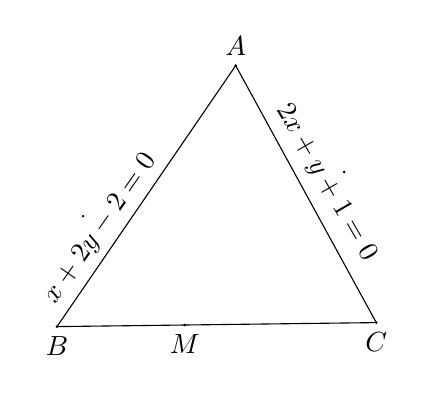
\begin{tikzpicture}[scale=.51]
					\coordinate (A) at (4.5,6.4);
					\coordinate (B) at (0.05,-0.1);
					\coordinate (C) at (8,0);
					\coordinate (P) at (3.23,-0.06);
					\coordinate (D) at (0.7,2.65);
					\coordinate (E) at (7.2,3.75);
					\draw (A) -- (B)--(C) -- (A);
					\fill (A) circle (1pt) node[above] {$A$};
					\fill (B) circle (1pt) node[below] {$B$};
					\fill (C) circle (1pt) node[below] {$C$};
					\fill (P) circle (1pt) node[below] {$M$};
					\fill (D) circle (1pt) node[rotate=55,below] {$x+2y-2=0$};
					\fill (E) circle (1pt) node[rotate=-60,below] {$2x+y+1=0$};
			\end{tikzpicture}}
			\begin{itemize}
				\item  Với $a = b \Rightarrow \overrightarrow{n} = (1;1)$.\\ 
				Phương trình $BC\colon x+y-3=0 \Rightarrow B(4;-1) C(-4;7)$.\\
				Ta có $\overrightarrow{BC}=(-8;8)$, $\overrightarrow{BM}=(-3;3)$ và $\overrightarrow{BC}=\dfrac{8}{3}\overrightarrow{BM}$.\\
				Nên $M$ thuộc đoạn $BC$.\\
				Gọi $D(x;y) \overrightarrow{DB}\cdot\overrightarrow{DC} = x^2 + (y-3)^2 - 32 \geq -32$.\\
				Vậy giá trị nhỏ nhất 
				$\overrightarrow{DB}\cdot\overrightarrow{DC} = -32 \Leftrightarrow D(0;3)$.
				\item Với $a = -b \Rightarrow \overrightarrow{n} = (1;-1)$.\\ 
				Phương trình $BC \colon x-y+1=0 \Rightarrow B(0;1)$, $C\left(-\dfrac{2}{3};\dfrac{1}{3}\right)$ (loại).\\
				Ta có $\overrightarrow{BC}=\left(-\dfrac{2}{3};-\dfrac{2}{3}\right)$, $\overrightarrow{BM}=(1;1)$ và $\overrightarrow{BC}=-\dfrac{2}{3}\overrightarrow{BM}$.\\
				Nên $M$ nằm ngoài thuộc đoạn $BC$, loại trường hợp này.\\
			\end{itemize}
		\end{enumerate}
	}
\end{ex}
\begin{ex}%[0H9V3-2]%[Dự án đề cương ba khối NH25-26-Dot 1- Nguyễn Hữu Đức]
	Cho ba điểm $A(-1 ; 4)$, $B(1 ; 1)$, $C(4 ;-2)$.	
	\begin{enumerate}
		\item  Viết phương trình tổng quát của đường thẳng $A B$.
		\item  Trên đoạn thẳng $B C$, lấy điểm $M$ sao cho diện tích tam giác $A B M$ gấp đôi diện tích tam giác $ACM$. Viết phương trình đường thẳng $AM$.
	\end{enumerate}
	\loigiai{
		\begin{enumerate}
			\item   Đường thẳng $AB$  nhận vectơ $\overrightarrow{AB}=(2 ;-3)$ là một vectơ chỉ phương, nên nhận $\overrightarrow{n}=(3 ; 2)$ là một vectơ pháp tuyến.\\		 	
			Phương trình tổng quát của $AB\colon 	3(x-1)+2(y-1)=0 \Leftrightarrow 3 x+2 y-5=0	$.
			\item\hfill\\
			\begin{center}
				\begin{tikzpicture}[scale=1,line cap=round,line join=round,font=\footnotesize,>=stealth,declare function={c=0.65;kc=0.15;cao=6*c+3*kc;dai=1.65*cao;dait=dai/3;}]
					\path
					(0,0) coordinate (B)
					($(B)+(60:2)$) coordinate (A)
					($(B)+(0:4)$) coordinate (C)
					($(B)!(A)!(C)$)  coordinate (H)
					($(B)!2/3!(C)$) coordinate (M)
					;
					\draw (A)--(B)--(C)--(A)--(H) (A)--(M);
					\draw (H)--++(0:0.2)--++(90:0.2)--++(180:0.2);
					\foreach \p/\r in {A/90, B/180, C/-90,H/-90, M/-90}
					\fill (\p) circle (1.25pt) node[shift={(\r:3mm)}]{$\p$};
				\end{tikzpicture}	 
			\end{center}
			
			Gọi $AH$ là đường cao tam giác $ABC $. Ta có	
			\begin{eqnarray*}
				&& S_{\triangle A B M}=\frac{A H \cdot B M}{2};\,  S_{\triangle A C M}=\dfrac{A H \cdot C M}{2}\\
				&& S_{\triangle A B M}=2 S_{\triangle A C M}\Rightarrow B M=2 C M \\
				&& \Rightarrow \overrightarrow{B M}=2 \overrightarrow{M C}\\
				&& \Rightarrow M(3 ;-1).
			\end{eqnarray*}		 
			Đường thẳng $AM$ nhận vectơ $\overrightarrow{AB}=(4 ;-5)$ là vectơ chỉ phương, có phương trình $$\heva{&x=-1+4 t \\&y=4-5 t.}$$			 	
	\end{enumerate}	}
\end{ex}
\begin{ex}[Trích đề kiểm tra Toán 10 GHKII-THPT Ea H'Leo - Đắk Lắk NH 2025-2025]%[ Quang Vinh NT]%[0H9V3-2]%
	Trong mặt phẳng $Oxy$, cho hình bình hành $ABCD$ có phương trình đường thẳng $AB\colon 3x + 2y + 1 = 0$, $AD\colon x - 3y - 18 = 0$ và điểm $M(1; -2)$ là trung điểm của cạnh $AB$. Viết phương trình cạnh $BC$.
	\loigiai{
		\begin{center}
			\begin{tikzpicture}[scale=.7,>=stealth, font=\footnotesize, line join=round, line cap=round]
				\path (0,0)coordinate(A)--++(8,0)coordinate(B) --++(1,4)coordinate(C)--++(-8,0)coordinate(D)	;
				\path 
				(A)--(B)coordinate[pos=0.5](M);	
				\draw (A)--(B)--(C)--(D)--cycle;
				\foreach \p/\q in {A/-90,B/-90,C/90,D/90,M/-90}
				{
					\path (\p) node[shift={(\q:3mm)}]{$\p$};
					\fill[black] (\p) circle (1pt);
				}		
			\end{tikzpicture}
		\end{center}
		Điểm $A$ là giao điểm $AB$ và $AD$ nên
		\[
		\heva{&3x + 2y + 1 = 0 \\&x - 3y - 18 = 0}\Leftrightarrow \heva{&x=3\\&y=-5.}
		\]		
		Vậy $A(3; -5)$.\\		
		Do $M$ là trung điểm của $AB$ nên
		\[
		\heva{&
			\dfrac{3 + x_B}{2} = 1 \\
			&\dfrac{-5 + y_B}{2} = -2
		}
		\Leftrightarrow \heva{&x_B=-1\\&y_B=1}
		\Rightarrow B(-1; 1).
		\]		
		Đường thẳng $AD\colon x - 3y - 18 = 0 \Rightarrow$ véc-tơ pháp tuyến $\overrightarrow{n} = (1; -3)$ \\
		Vì $BC \parallel AD$ nên phương trình $BC$ có dạng $x - 3y + d = 0$.\\
		Do $B(-1; 1)$ thuộc $BC$ nên  $-1 - 3\cdot 1 + d = 0 \Rightarrow d = 4$.\\
		Vậy phương trình đường thẳng $BC$ là $x - 3y + 4 = 0.$
	}
\end{ex}

\begin{ex}[Trích đề kiểm tra Toán 10 GHKII-THPT Chuyên Lương Thế Vinh-Đồng Nai NH 2025-2025]%[ Phạm Văn Long]%[0H9V3-6]%
	Trong mặt phẳng tọa độ $Oxy$, cho đường thẳng $d$ đi qua $A(1;1)$ và có $\overrightarrow{u}=(2;-1)$ là một véc-tơ chỉ phương.
	\begin{enumerate}
		\item Viết phương trình tham số của đường thẳng $d$.
		\item Tìm tọa độ điểm $M$ thuộc đường thẳng $d$ sao cho $OM=3\sqrt{2}$.
	\end{enumerate}
	\loigiai{
		\begin{enumerate}
			\item Phương trình tham số đường thẳng $d$ đi qua $A(1 ; 1)$ và có $\overrightarrow{u}=(2 ;-1)$ là một véc-tơ chỉ phương là		
			$$\heva{&x=1+2t \\&y=1-t}(t \in \mathbb{R}).$$
			\item Vì $M$ thuộc đường thẳng $\heva{&x=1+2t\\&y=1-t}$ nên tọa độ điểm $M$ có dạng $M(1+2t;1-t)$.\\
			Ta có \allowdisplaybreaks
			\begin{eqnarray*}
				OM=3 \sqrt{2} &\Leftrightarrow& OM^2=18\\
				&\Leftrightarrow& (1+2 t)^2+(1-t)^2=18\\
				&\Leftrightarrow& 5t^2+2 t-16=0 \\
				&\Leftrightarrow& t=-2 \text { hoặc } t=\dfrac{8}{5}.
			\end{eqnarray*}
			\begin{itemize}
				\item Với $t=-2$ thì $M(-3;3)$.
				\item Với $t=\dfrac{8}{5}$ thì $M\left(\dfrac{21}{5};-\dfrac{3}{5}\right)$.
			\end{itemize}	
		\end{enumerate}
	}
\end{ex}
\begin{ex}[Trích đề kiểm tra Toán 10 GHKII NH2024-2025]%[-Nguyễn Tài Tuệ] %[0H9H3-8]%
	Trong mặt phẳng tọa độ $O x y$, người ta đặt máy phát tín hiệu tại $A(1 ; 1)$ và đặt máy thu tương ứng trên đường thẳng $x+y+2=0$. Biết đặt máy thu tại điểm $M(a ; b)$ sẽ bắt được tín hiệu sớm nhất vì ở gần máy phát nhất. Tìm $a+b$.
	\loigiai{
		Tại điểm $M(a;b)$ bắt được tín hiệu sớm nhất khi $M$ là hình chiếu của $A$ lên đường thẳng $d\colon x+y+2=0$.\\
		Đường thẳng $\Delta $ vuông góc với đường thẳng $d$ có dạng $x-y+c=0$.\\
		Vì $A\in \Delta$ nên $1-1+c=0\Leftrightarrow c=0$.\\
		Do đó phương trình đường thẳng $\Delta\colon x-y=0$.\\
		Tọa độ điểm $M$ là nghiệm của hệ phương trình $\heva{&x+y+2=0\\&x-y=0}\Leftrightarrow \heva{&x=-1\\&y=-1.}$\\
		Do đó $a+b=-2$.
	}
\end{ex}
\begin{ex}[Trích đề kiểm tra Toán 10 GHKII NH2024-2025]%[Nguyễn Tài Tuệ]%[0H9V3-2]%
	Cho ba điểm $A(-1 ; 4)$, $B(1 ; 1)$, $C(4 ;-2)$.	
	\begin{enumerate}
		\item  Viết phương trình tổng quát của đường thẳng $A B$.
		\item  Trên đoạn thẳng $B C$, lấy điểm $M$ sao cho diện tích tam giác $A B M$ gấp đôi diện tích tam giác $ACM$. Viết phương trình đường thẳng $AM$.
	\end{enumerate}
	\loigiai{
		\begin{enumerate}
			\item   Đường thẳng $AB$  nhận véctơ $\overrightarrow{AB}=(2 ;-3)$ là một véctơ chỉ phương, nên nhận $\overrightarrow{n}=(3 ; 2)$ là một véctơ pháp tuyến.\\		 	
			Phương trình tổng quát của $AB\colon 	3(x-1)+2(y-1)=0 \Leftrightarrow 3 x+2 y-5=0	$.
			\item\hfill\\
			\begin{center}
				\begin{tikzpicture}[scale=1,line cap=round,line join=round,font=\footnotesize,>=stealth,declare function={c=0.65;kc=0.15;cao=6*c+3*kc;dai=1.65*cao;dait=dai/3;}]
					\path
					(0,0) coordinate (B)
					($(B)+(60:2)$) coordinate (A)
					($(B)+(0:4)$) coordinate (C)
					($(B)!(A)!(C)$)  coordinate (H)
					($(B)!2/3!(C)$) coordinate (M)
					;
					\draw (A)--(B)--(C)--(A)--(H) (A)--(M);
					\draw (H)--++(0:0.2)--++(90:0.2)--++(180:0.2);
					\foreach \p/\r in {A/90, B/180, C/-90,H/-90, M/-90}
					\fill (\p) circle (1.25pt) node[shift={(\r:3mm)}]{$\p$};
				\end{tikzpicture}	 
			\end{center}
			
			Gọi $AH$ là đường cao tam giác $ABC $. Ta có	
			\begin{eqnarray*}
				&& S_{\triangle A B M}=\frac{A H \cdot B M}{2};\,  S_{\triangle A C M}=\dfrac{A H \cdot C M}{2}\\
				&& S_{\triangle A B M}=2 S_{\triangle A C M}\Rightarrow B M=2 C M \\
				&& \Rightarrow \overrightarrow{B M}=2 \overrightarrow{M C}\\
				&& \Rightarrow M(3 ;-1).
			\end{eqnarray*}		 
			Đường thẳng $AM$ nhận véctơ $\overrightarrow{AB}=(4 ;-5)$ là véctơ chỉ phương, có phương trình $$\heva{&x=-1+4 t \\&y=4-5 t.}$$			 	
	\end{enumerate}	}
\end{ex}

